\documentclass[10pt]{article}
\usepackage{graphicx}
\usepackage[margin=1.5cm]{geometry}
\usepackage{amsmath}
\def\brcurs{{\mbox{$\resizebox{.16in}{.08in}{
\includegraphics{BoldR}}$}}}
\def\rcurs{{\mbox{$\resizebox{.16in}{.08in}{
\includegraphics{ScriptR}}$}}}

\begin{document}
\twocolumn

\title{Thursday Warm-up: Electric Fields in Matter}
\author{Prof. Jordan C. Hanson}

\maketitle

\section{Memory Bank}

\small

\begin{itemize}
\item \textbf{Relative voltage}:
\begin{equation}
V = - \int_a^{b} \mathbf{E} \cdot d\mathbf{l}
\end{equation}
\item \textbf{The electric displacement}:
\begin{equation}
\mathbf{D} = \epsilon_0 \mathbf{E} + \mathbf{P}
\end{equation}
\item \textbf{Gauss' Law for electric displacement}:
\begin{equation}
\oint \mathbf{D} \cdot d\mathbf{a} = Q_{\rm f,enc}
\end{equation}
\item \textbf{Linear dielectric materials}:
\begin{align}
\mathbf{P} &= \epsilon_0\chi_{\rm e} \mathbf{E} \\
\mathbf{D} &= \epsilon_0 \left(1+\chi_{\rm e}\right)\mathbf{E} \\
\mathbf{D} &= \epsilon \mathbf{E} \\
\epsilon_{\rm r} &= \epsilon/\epsilon_0 = 1+\chi_{\rm e}
\end{align}
\end{itemize}

\begin{figure}
\centering
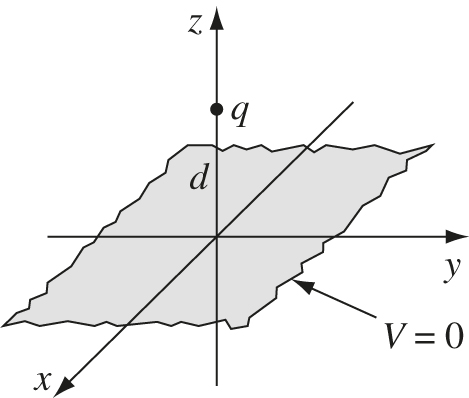
\includegraphics[width=0.2\textwidth]{figures/3_10.jpg} \hspace{0.5cm}
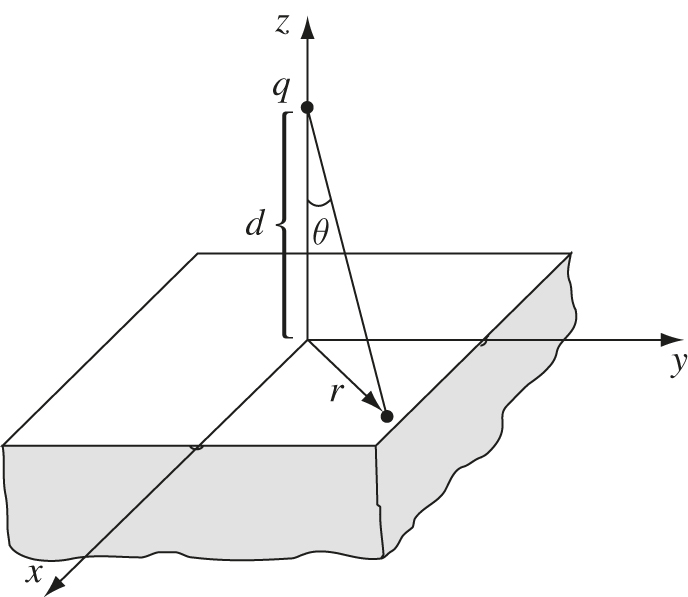
\includegraphics[width=0.24\textwidth]{figures/4_31.jpg}
\caption{\label{fig:1} (Left) A free charge above a conductor filling space with $z<0$. (Right) A free charge above a linear dielectric filling space with $z<0$.}
\end{figure}

\section{Linear Dielectric Materials}

\begin{enumerate}
\item Consider Fig. \ref{fig:1} (left).  Using the Method of Images, calculate $V(x,y,z)$ and $\mathbf{E}(x,y,z)$ for $z\geq 0$. \\ \vspace{4cm}
\item Consider Fig. \ref{fig:1} (left).  (a) Calculate the induced surface charge distribution. (b) Calculate the total induced charge. \\ \vspace{3.5cm}
\item Consider Fig. \ref{fig:1} (right).  The entire region for $z<0$ is filled with uniform linear dielectric material with susceptibility $\chi_e$.  Calculate the force on a point charge $q$ a distance $d$ above the origin.
\begin{itemize}
\item First, write an expression for the bound surface charge in terms of $E_z$, the z-component of the total field just inside the dielectric. \\ \vspace{2cm}
\item (a) Write the z-component of the field contribution from $q$ at a point $r$ on the surface. (b) Using Gauss' law, write the field contribution from the surface bound charge. \\ \vspace{2cm}
\item (a) Solve for the surface bound charge. (b) Calculate the \textit{total} bound charge, $q_b$. \\ \vspace{2cm}
\item What is the force between $q$ and $q_b$?  How does this compare to the force between $q$ and the conductor?
\end{itemize}
\end{enumerate}

\end{document}
